\documentclass{standalone}
\usepackage[english]{babel}
% https://tex.stackexchange.com/questions/570303/use-blacktriangleright-as-itemize-label
\usepackage{amssymb} % for black triangleright

\renewcommand{\labelitemi}{$\textcolor{SwitchColor}{\bullet}$}
\renewcommand{\labelitemii}{$\textcolor{SwitchColor}{\blacktriangleright}$}
\renewcommand{\labelitemiii}{$\textcolor{SwitchColor}{\blacksquare}$}

% https://tex.stackexchange.com/questions/525959/prevent-latex-from-stretching-math
\setlength{\thinmuskip}{1\thinmuskip}
\setlength{\medmuskip}{1\medmuskip}
\setlength{\thickmuskip}{1\thickmuskip}

\usepackage{csquotes}
\usepackage{xcolor}
% \usepackage{anyfontsize}
\usepackage[export]{adjustbox}
% \usepackage[]{enumitem}
\usepackage{nicematrix}
\usepackage{tikz}
\usetikzlibrary{arrows.meta,positioning}
\usetikzlibrary{graphs}
\usetikzlibrary{patterns}
\usetikzlibrary{shadings}
\usetikzlibrary{mindmap, shadows, backgrounds} % , calc

\definecolor{PrimaryColor}{HTML}{003BAB}
\definecolor{PrimaryColorDimmed}{HTML}{9CC6D3}
\definecolor{SecondaryColor}{HTML}{FFF77B}
\definecolor{SecondaryColorDimmed}{HTML}{EDE7A9}
\colorlet{BoxColor}{gray!10!white}

% colored bold
% \newcommand\alert[1]{\textcolor{SwitchColor}{\textbf{#1}}}
\newcommand\alert[1]{\textcolor{SwitchColor}{#1}}

\newlength{\leveldistance}
\setlength{\leveldistance}{25cm}

\begin{document}
  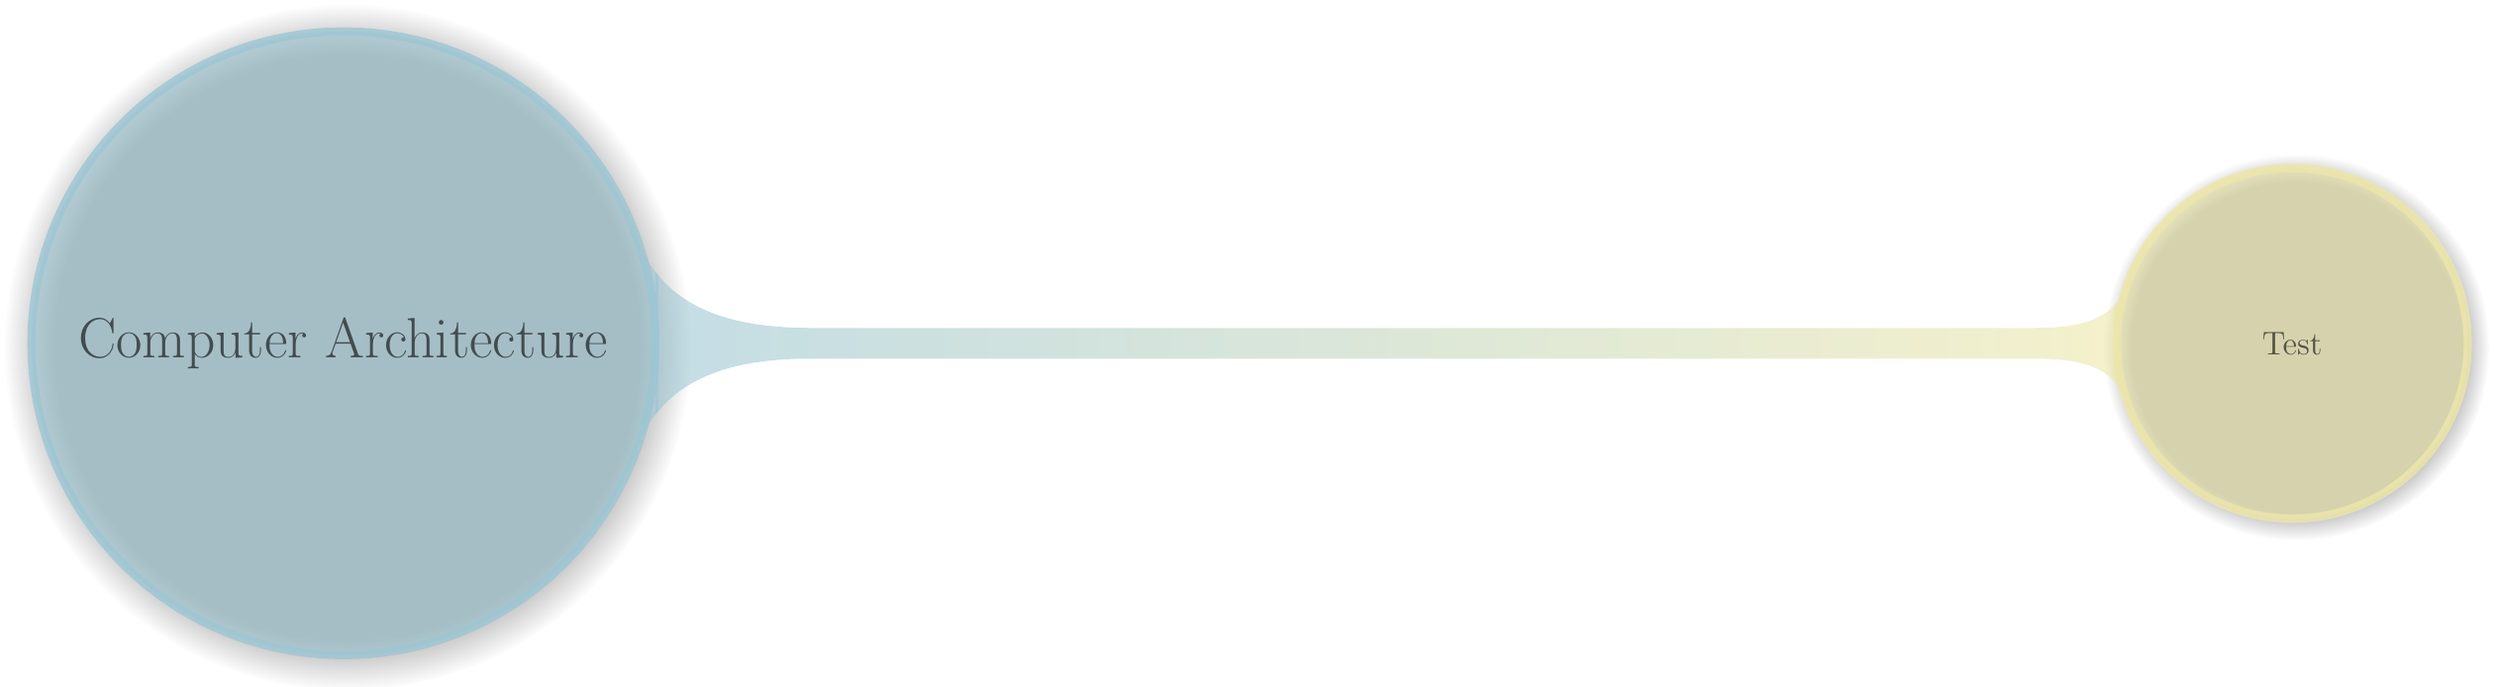
\begin{tikzpicture}[
      auto,
      huge mindmap,
      fill opacity=0.6,
      draw opacity=0.8,
      concept color = PrimaryColorDimmed,
      every annotation/.style={fill=BoxColor, draw=none, align=center, fill = BoxColor, text width = 2cm},
      grow cyclic,
      level 1/.append style = {
        concept color=SecondaryColorDimmed,
        level distance=\leveldistance,
        sibling angle=360/\the\tikznumberofchildren,
        % https://tex.stackexchange.com/questions/501240/trying-to-use-the-array-environment-inside-a-tikz-node-with-execute-at-begin-no
        execute at begin node=\definecolor{SwitchColor}{named}{SecondaryColor},
      },
      level 2/.append style = {
        concept color=PrimaryColorDimmed,
        level distance=\leveldistance / 2,
        sibling angle=30,
        execute at begin node=\definecolor{SwitchColor}{named}{PrimaryColor},
      },
      level 3/.append style = {
        concept color=SecondaryColorDimmed,
        level distance=\leveldistance / 3,
        execute at begin node=\definecolor{SwitchColor}{named}{SecondaryColor},
      },
      level 4/.append style = {
        concept color=PrimaryColorDimmed,
        level distance=\leveldistance / 4,
        execute at begin node=\definecolor{SwitchColor}{named}{PrimaryColor},
      },
      level 5/.append style = {
        concept color=SecondaryColorDimmed,
        level distance=\leveldistance / 5,
        execute at begin node=\definecolor{SwitchColor}{named}{SecondaryColor},
      },
      level 6/.append style = {
        concept color=PrimaryColorDimmed,
        level distance=\leveldistance / 6,
        execute at begin node=\definecolor{SwitchColor}{named}{PrimaryColor},
      },
      level 7/.append style = {
        concept color=SecondaryColorDimmed,
        level distance=\leveldistance / 7,
        execute at begin node=\definecolor{SwitchColor}{named}{SecondaryColor},
      },
      level 8/.append style = {
        concept color=PrimaryColorDimmed,
        level distance=\leveldistance / 8,
        execute at begin node=\definecolor{SwitchColor}{named}{PrimaryColor},
      },
      concept connection/.append style = {
        color = BoxColor,
      },
  ]
  % damit Annotationen nicht auch eine Drop Shadow erhalten
  \begin{scope}[
      every node/.style = {concept, circular drop shadow}, % draw=none
      every child/.style={concept},
    ]
  \node (ca) at (current page.center) {Computer Architecture}
  child {
    node {Test}
  };
  \end{scope}
  % ┌───────────────────┐
  % │ Verbindungslinien │
  % └───────────────────┘
  \begin{pgfonlayer}{background}
  % \draw [concept connection]
  %     (commoncasefast) edge (amdahl)
  %     (branchpredictionbuffer) edge (2bitpredictor)
  %     (loadusedatahazard) edge (forwarding)
  %     (datahazardsforbranches) edge (forwarding);
  \end{pgfonlayer}
  % ┌──────────────┐
  % │ Annotationen │
  % └──────────────┘
  % https://tex.stackexchange.com/questions/302976/node-positioning-middle-point-mind-map-connection-bar
  % \path (measuringexecutiontime) -- node[annotation, above, align=center, pos=0.01] {Similiar to \textbf{Response Time:} How long it takes to do a task} (ca);
  % \path (performance) -- node[annotation, above, align=center, pos=0.01] {Similiar to \textbf{Throughput}: Total work done per time unit (e.g. tasks, transactions\ldots / per hour)} (ca);
  % \path (elapsedtime) -- node[annotation, above, align=center, pos=0.01] {Also called \textbf{Wall Clock Time} or \textbf{Real Time}} (ca);
  % \path (cputime) -- node[annotation, above, align=center, pos=0.01] {Also called \textbf{User Time}} (ca);
  % % \path (branchpredictionbuffer) -- node[annotation, below, align=center, pos=-0.06] {Also called Branch History Table} (ca);
  % \path (multicycle) -- node[annotation, above, align=center, pos=0.01] {Optimize space} (ca);
  % \path (pipelining) -- node[annotation, above, align=center, pos=0.01] {Optimize time} (ca);
  % \node [annotation, below] at (ca.south) {This mindmap is provided without guarantee of correctness and completeness!};
  \end{tikzpicture}
\end{document}
